\documentclass{article}

\usepackage{graphicx}
\usepackage{tikz}
\usepackage{tikzsymbols}
\usetikzlibrary{calc,patterns,shapes.geometric}
\pagestyle{empty}
\usepackage[margin=0pt]{geometry}
\geometry{papersize={14in,12in}}

\def\centerarc[#1](#2)(#3:#4:#5){\draw[#1] ($(#2)+({#5*cos(#3)},{#5*sin(#3)})$) arc (#3:#4:#5);}

\begin{document}
	\begin{figure}
		\centering
		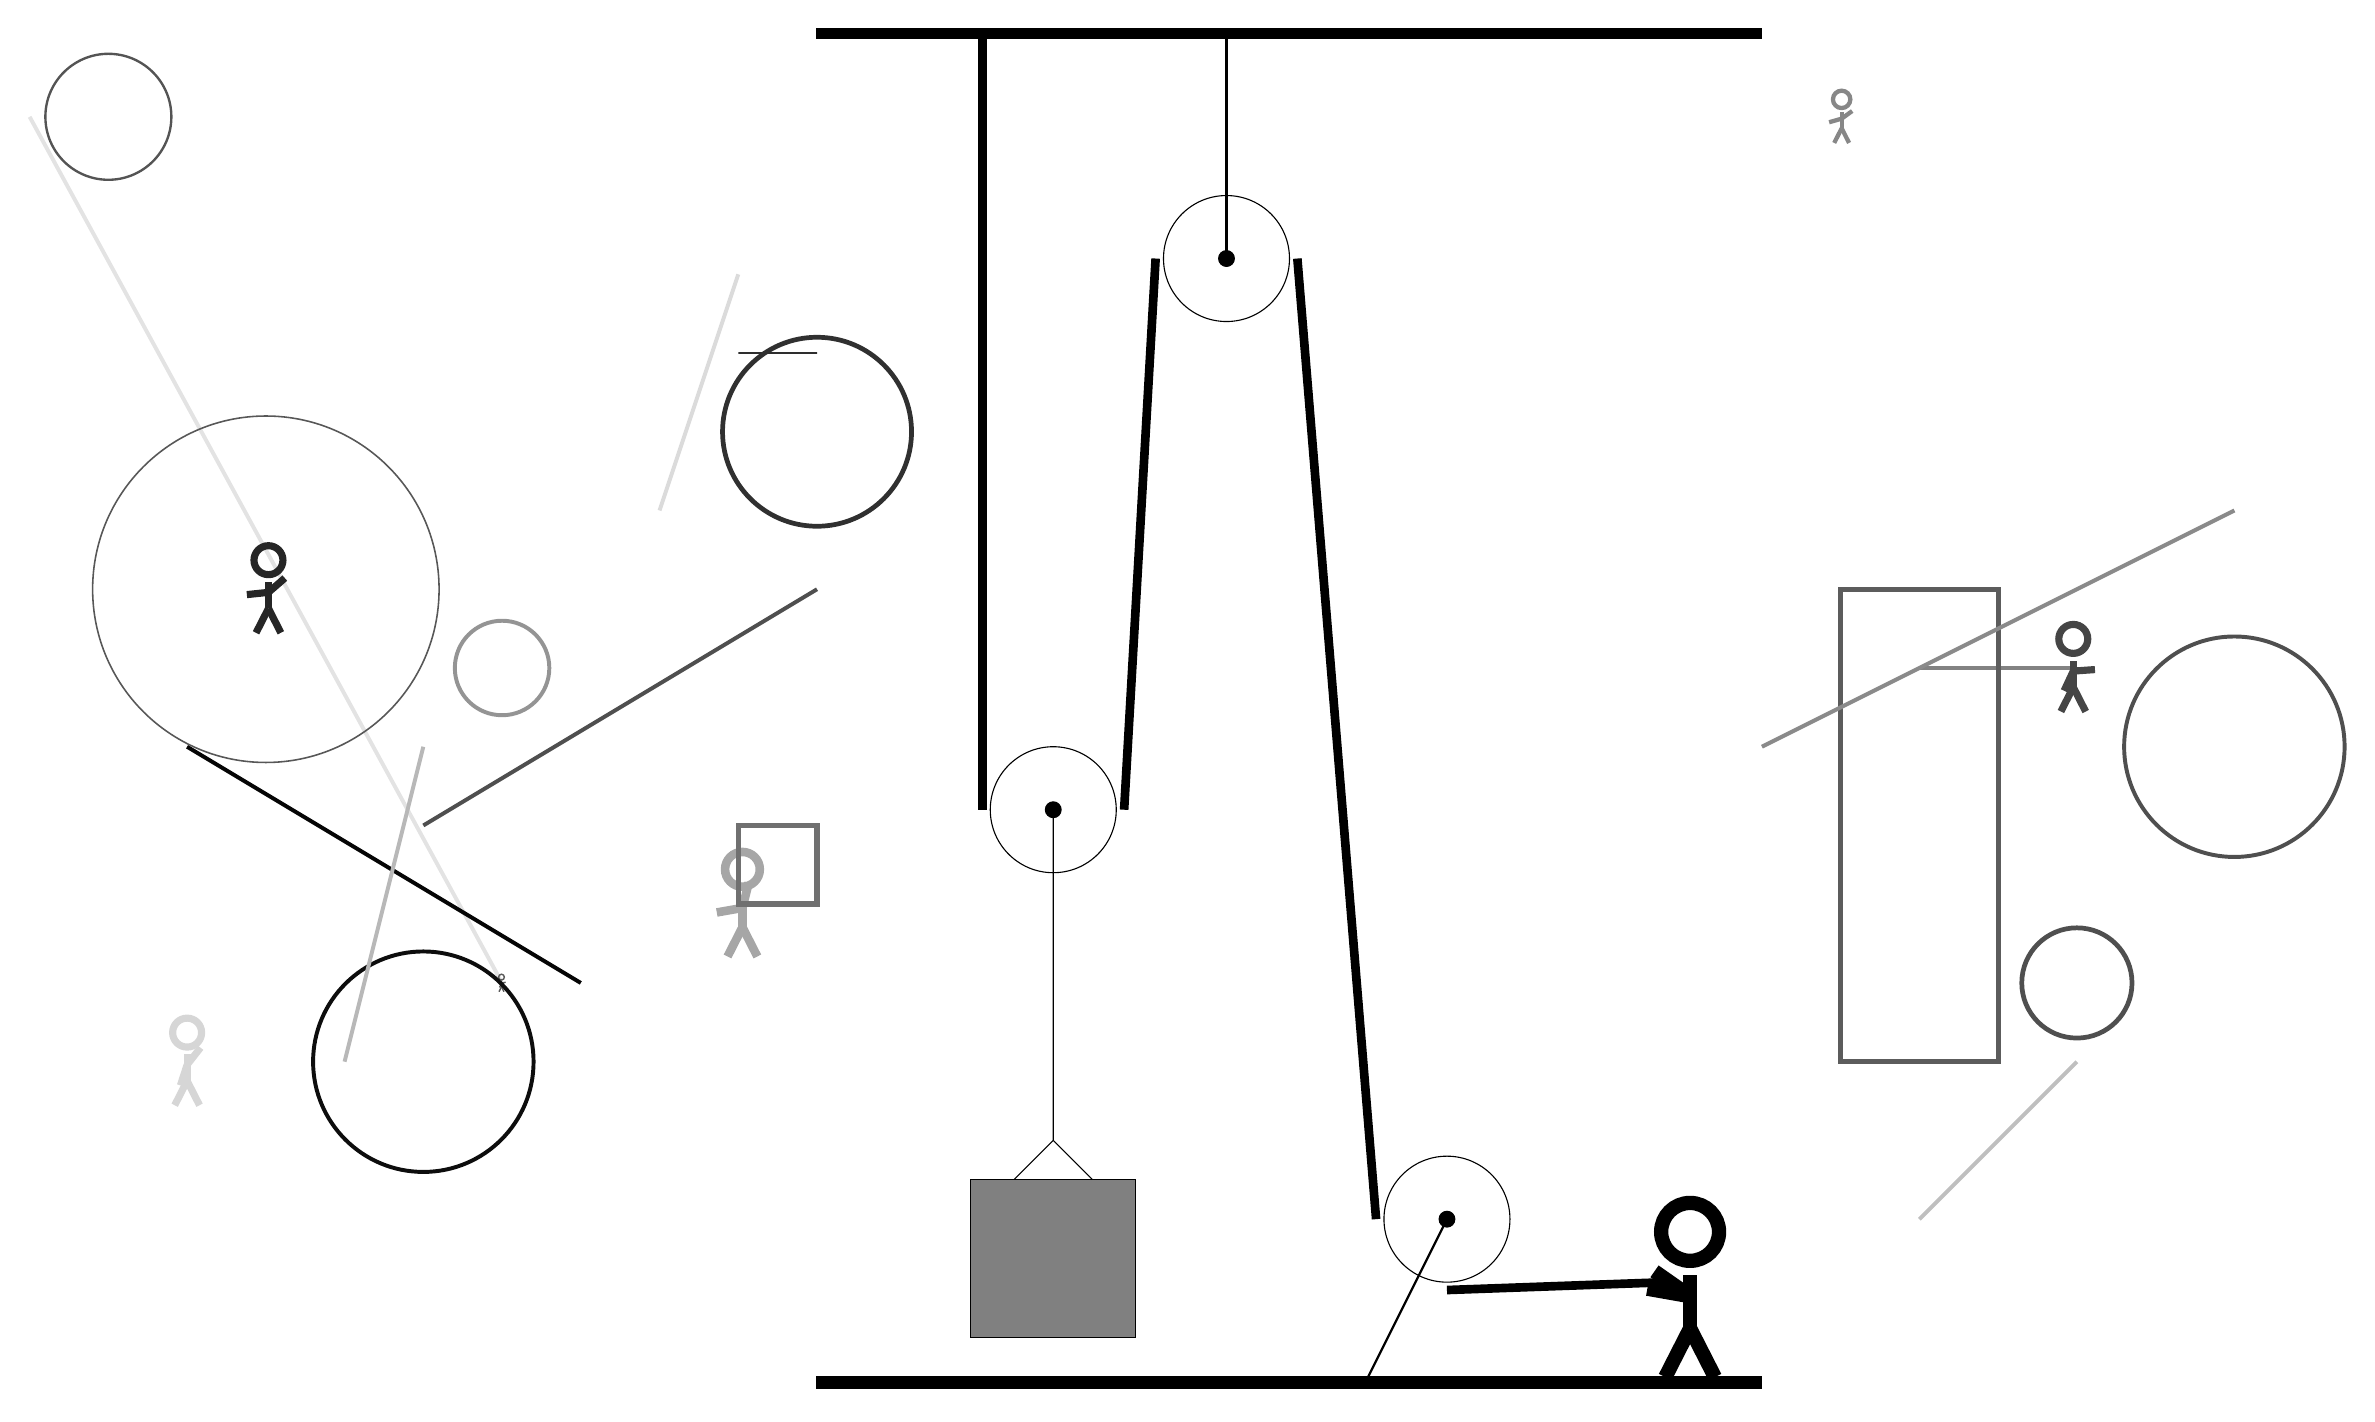
\begin{tikzpicture}
			%%%%% START %%%%%
			
			\draw[fill=black] (-2, 14) rectangle (10, 14.125);
			
			\draw (3.2, 11.2) circle (0.8);
			\draw[fill=black] (3.2, 11.2) circle (0.1);
			\draw[thick] (3.2, 11.2) -- (3.2, 14);
			
			\draw (6, -1) circle (0.8);
			\draw[fill=black] (6, -1) circle (0.1);
			\draw[thick] (6, -1) -- (5, -3);
			
			\draw (1, 4.2) circle (0.8);
			\draw[fill=black] (1, 4.2) circle (0.1);
			
			\draw (1, 4.2) -- (1, 0) -- (0.5, -0.5);
			\draw (1, 0) -- (1.5, -0.5);
			\draw[fill=black!50] (-0.05, -0.5) rectangle (2.05, -2.5);
			
			\draw[line width=0.5mm, color=black!49](14, 6) -- (12, 6);
			
			\draw[line width=0.6mm, color=black!64] (11, 1) rectangle (13, 7);
			\draw [line width=0.3mm, color=black!83](13, 11) circle (0.0);
			\draw [line width=0.5mm, color=black!69](16, 5) circle (1.4);
			\node[line width=0.5mm, color=black!35] at (-3, 3) {\Strichmaxerl[6][10][76]};
			\draw[line width=0.5mm, color=black!11](-6, 2) -- (-12, 13);
			
			\node[line width=0.7mm, color=black!73] at (14, 6) {\Strichmaxerl[5][65][4]};
			
			\draw[line width=0.5mm, color=black!25](14, 1) -- (12, -1);
			\draw[line width=0.5mm, color=black!14](-4, 8) -- (-3, 11);
			
			\draw[line width=0.7mm, color=black!56] (-3, 4) rectangle (-2, 3);
			\node[line width=0.2mm, color=black!64] at (-6, 2) {\Strichmaxerl[1][63][19]};
			\node[line width=0.3mm, color=black!85] at (-9, 7) {\Strichmaxerl[5][6][41]};
			\draw[line width=0.5mm, color=black!98](-5, 2) -- (-10, 5);
			\draw [line width=0.5mm, color=black!95](-7, 1) circle (1.4);
			\draw [line width=0.4mm, color=black!28](12, 3) circle (0.0);
			\node[line width=0.3mm, color=black!16] at (-10, 1) {\Strichmaxerl[5][72][52]};
			
			\draw [line width=0.3mm, color=black!67](-11, 13) circle (0.8);
			\draw[line width=0.2mm, color=black!82] (-3, 10) rectangle (-2, 10);
			\draw [line width=0.2mm, color=black!66](-9, 7) circle (2.2);
			\draw[line width=0.5mm, color=black!46](10, 5) -- (16, 8);
			\draw [line width=0.6mm, color=black!69](14, 2) circle (0.7);
			
			\draw [line width=0.5mm, color=black!42](-6, 6) circle (0.6);
			\draw [line width=0.6mm, color=black!81](-2, 9) circle (1.2);
			\node[line width=0.4mm, color=black!47] at (11, 13) {\Strichmaxerl[3][16][36]};
			\draw[line width=0.5mm, color=black!28](-7, 5) -- (-8, 1);
			
			\draw[line width=0.5mm, color=black!69](-7, 4) -- (-2, 7);
			
			
			\draw[line width=1.1mm] (0.1, 14) -- (0.1, 4.2);
			\centerarc[line width=1.1mm](1, 4.2)(180:360:0.9);
			\draw[line width=1.1mm](1.9, 4.2) -- (2.3, 11.2);
			\centerarc[line width=1.1mm](3.2, 11.2)(0:180:0.9);
			\draw[line width=1.1mm](4.1, 11.2) -- (5.1, -1);
			\centerarc[line width=1.1mm](6, -1)(180:270:0.9);
			\draw[line width=1.1mm](6, -1.9) -- (8.8, -1.8);
			
			\node at (9, -1.9) {\Strichmaxerl[10][-35][170]};
			
			\draw[fill=black] (-2, -3) rectangle (10, -3.15);
			
			%%%%% END %%%%%
		\end{tikzpicture}
	\end{figure}	
\end{document}